\documentclass{standalone}
\usepackage{tikz}
%------------tikz Setup------------

\tikzstyle{ball} = [circle,shading=ball, ball color=black,
    minimum size=1mm,inner sep=1.3pt]
\tikzstyle{miniball} = [circle,shading=ball, ball color=black,
    minimum size=1mm,inner sep=0.5pt]
\tikzstyle{mminiball} = [circle,shading=ball, ball color=black,
    minimum size=0.6mm,inner sep=0.1pt]
\usetikzlibrary{arrows.meta}
\usetikzlibrary{angles, quotes}
\tikzset{>={Latex[length=2mm,width=1.5mm]}}
\tikzset{->-/.style={decoration={markings, mark=at position #1 with
  {\arrow{>}}},postaction={decorate}}}
\usetikzlibrary{decorations.pathmorphing}
\usetikzlibrary{decorations.pathreplacing}
\usetikzlibrary{arrows.meta,calc}
\usetikzlibrary{bending}
\usetikzlibrary{decorations.markings,shapes.geometric}
\tikzset{->-/.style={decoration={markings, mark=at position #1 with
  {\arrow{>}}},postaction={decorate}}}
\tikzset{-|-/.style={decoration={markings, mark=at position #1 with
  {\arrow{stealth}}},postaction={decorate}}}
\tikzset{movearrow/.style 2 args ={
        decoration={markings,
    mark= at position {#1} with {\arrow{#2}} ,
        },
        postaction={decorate}
    }
}


\begin{document}
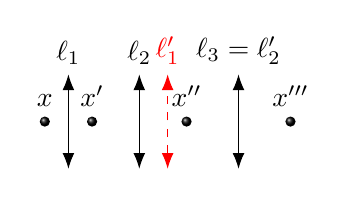
\begin{tikzpicture}
\begin{scope}[scale=0.6]
    %lines
    \draw [<->] (-1,-1) -- (-1,1);
    \draw [<->] (0.5,-1) -- (0.5,1);
    \draw [<->] (2.6,-1) -- (2.6,1);
    \draw [<->, dashed, red] (1.1,-1) -- (1.1,1);
    %labels
    \node[above] at (-1,1) {$\ell_1$};
    \node[above] at (0.5,1) {$\ell_2$};
    \node[above] at (2.6,1) {$\ell_3=\ell_2'$};
    \node[above,red] at (1.1,1) {$\ell_1'$};
    %points
    \node[ball, label={$x$}] (x) at (-1.5,0) {};
    \node[ball, label={$x'$}] (x') at (-0.5,0) {};
    \node[ball, label={$x''$}] (x'') at (1.5,0) {};
    \node[ball, label={$x'''$}] (x''') at (3.7,0) {};
\end{scope}
\end{tikzpicture}
\end{document}